\chapter{ম্যাট্রিক্স এক্সপোনেন্সিয়েশন}

\section{শুরুর কথা}

\noindent নামটা শুনতে কঠিন মনে হলেও ম্যাট্রিক্স এক্সপোনেন্সিয়েশন আসলে তেমন কঠিন কিছু না। ম্যাট্রিক্স সম্পর্কে কমবেশি সবারই জানা থাকার কথা। তারপরেও যারা এ সম্পর্কে জানো না তারা ম্যাট্রিক্সকে 2D অ্যারের মত চিন্তা করতে পার। বাইরে থেকে দুটি একইরকমই দেখতে। যদি কোন ম্যাট্রিক্সের $n$ টি সারি আর $m$ টি কলাম থাকে তাহলে ম্যাট্রিক্সটিকে $n \times m$ ম্যাট্রিক্স বলা হয়। যেমন নিচের ম্যাট্রিক্সটি একটি $2 \times 3$ ম্যাট্রিক্স।
$$
\begin{pmatrix}
1 & 3 & 2\\
9 & 0 & 7
\end{pmatrix}
$$

\noindent ঠিক অ্যারের মতই কোন ম্যাট্রিক্স $A$ এর $i$ তম সারির $j$ তম সংখ্যাকে $A_{ij}$ দিয়ে প্রকাশ করা হয়। যেমন উপরের ম্যাট্রিক্সের জন্য $A_{11} = 1$, আবার $A_{23} = 7$। ম্যাট্রিক্সের যোগ, বিয়োগও সম্ভব, তবে তুমি একটি $n \times m$ ম্যাট্রিক্সের সাথে আরেকটি $n \times m$ ম্যাট্রিক্সই যোগ বা বিয়োগ করতে পারবে। এক্ষেত্রে $A$ এবং  $B$ যোগ করে $C$ পাওয়া গেলে $C_{ij} = A_{ij} + B_{ij}$ হতে হবে। যেমন

$$
\begin{pmatrix}
1 & 3\\
9 & 0
\end{pmatrix}
+
\begin{pmatrix}
2 & -1\\
3 & 1
\end{pmatrix}
=
\begin{pmatrix}
1 + 2 & 3 - 1\\
9 + 3 & 0 + 1
\end{pmatrix}
$$

\noindent তবে সবচেয়ে অদ্ভুত হচ্ছে ম্যাট্রিক্সের গুন। গুনের ক্ষেত্রে একটি $n \times m$ ম্যাট্রিক্সের সাথে কেবল একটা $m \times l$ ম্যাট্রিক্স গুন করতে পারবে এবং  গুণফল হবে একটা $n \times l$ ম্যাট্রিক্স। অর্থাৎ প্রথম ম্যাট্রিক্সের কলাম সংখ্যা আর দ্বিতীয় ম্যাট্রিক্সের সারি সংখ্যা সমান হতে হবে। $C$ যদি $A$ এবং $B$ ম্যাট্রিক্সের গুণফল হয় তাহলে

\begin{equation}
  \label{mult:1}
  C_{ij} = \sum_{k = 1}^{m} A_{ik} B_{kj}
\end{equation}

যেমন ধর,

$$
\begin{pmatrix}
1 & 3 & 2\\
9 & 0 & 7
\end{pmatrix}
\begin{pmatrix}
5 & 6 & 0 & 3 \\
0 & 2 & -1 & 1\\
1 & 1 & 4 & -1
\end{pmatrix} =
\begin{pmatrix}
5 & 6 & 7 & 8\\
9 & 10 & 12 & 13
\end{pmatrix}
$$

\noindent এখানে $2 \times 3$ ম্যাট্রিক্সের সাথে $3 \times 4$ ম্যাট্রিক্স গুন করে $2 \times 4$ ম্যাট্রিক্স পাওয়া গিয়েছে। তবে গুণফলটা আসলে কীভাবে বের হল সেটা হয়ত \eqref{mult:1} সমীকরণ দিয়ে ভালভাবে কল্পনা করা একটু কঠিন। এজন্য আমাদের ভেক্টর-ভেক্টর গুণফল ভালভাবে বুঝতে হবে আগে।

\section{ভেক্টর-ভেক্টর গুণফল}
\noindent $n \times 1$ বা $1 \times n$ আকারের ম্যাট্রিক্সগুলোর একটি বিশেষ নাম আছে। এদের কে ভেক্টর বলা হয়। স্বভাবতই, $1 \times n$ ম্যাট্রিক্স রো ভেক্টর (row vector) নামে পরিচিত, কারণ এটি অনেকটা রো এর মতই দেখতে। একই ভাবে $n \times 1$ ম্যাট্রিক্স কলাম ভেক্টর (column vector) নামে পরিচিত, কারণ এটি অনেকটা কলামের মত দেখতে। সাইজ দেখেই বুঝতে পারছ, $n$ সাইজের একটি রো ভেক্টর এর সাথে $n$ সাইজের একটি কলাম ভেক্টর গুন করলে $1 \times 1$ ম্যাট্রিক্স পাওয়া যাবে। এই $1 \times 1$ ম্যাট্রিক্সকে ম্যাট্রিক্স না বলে একটা সংখ্যা হিসেবেই কল্পনা করা যায়। এই যে আমরা একটা রো ভেক্টর এর সাথে কলাম ভেক্টরের গুন করলাম এটারও একটা বিশেষ নাম আছে কিন্তু। এটাকেই বলা হয় ম্যাট্রিক্সের ডট প্রডাক্ট। এই গুণফলকে সংজ্ঞায়িত করা হয়েছে এভাবে:
$$
\begin{pmatrix}
a_1 \ a_2 \ a_3\\
\end{pmatrix}
\begin{pmatrix}
b_1 \\
b_2 \\
b_3
\end{pmatrix} =
a_1 b_1 + a_2 b_2 + a_3 b_3
$$

\noindent এখানে আমরা $3$ সাইজের ভেক্টর এর জন্য দেখলাম, কিন্তু অন্য ভেক্টর এর জন্যও একি ভাবে বের করা যাবে। সোজা কথায় রো ভেক্টরের $i$ তম সংখ্যার সাথে কলাম ভেক্টরের $i$ তম সংখ্যা গুন দিয়ে সবগুলোর যোগফল নিলেই হবে। আমরা একটু আগে যে ম্যাট্রিক্স গুণফল শিখেছিলাম তার চেয়ে কিন্তু এটা ভিজুয়ালাইজ করা বেশ সহজ।

\noindent একটা জিনিশ খেয়াল কর। একটি $n \times m$ ম্যাট্রিক্স কিন্তু $n$ টা রো ভেক্টর নিচে নিচে সাজালেই পাওয়া যাবে। একইভাবে একটি $n \times m$ ম্যাট্রিক্সকে $m$ টি কলাম ভেক্টর পাশাপাশি সাজালেই পাওয়া যায়। অর্থাত যেকোনো ম্যাট্রিক্সকেই কিছু রো ভেক্টর বা কিছু কলাম ভেক্টর এর সমাহার হিসেবে চিন্তা করা যায়।

\noindent এবার আমরা ম্যাট্রিক্স গুনকে একটু ভিন্ন ভাবে দেখতে পারি। $A$ এর $i$ তম রো এবং $B$ এর $j$ তম কলাম ডট গুন করলেই আমরা $AB$ এর $(i, j)$ অবস্থানের মান বের করতে পারব। নিচের ম্যাট্রিক্সটি দেখ।

\begin{figure}[h]
  \centering
  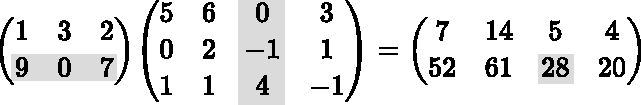
\includegraphics[scale=0.8]{./img/mat-expo/multiply.pdf}
\end{figure}

\noindent ধর আমরা গুণফলের $(2, 3)$ অবস্থানের মান বের করতে চাই। তাহলে বামপাশের ম্যাট্রিক্সের $2$ তম রো এবং ডান পাশের ম্যাট্রিক্সের $3$ তম কলাম নিব। ছবিতে রো আর কলাম দুটি মার্ক করে দিয়েছি। এবার এই রো ভেক্টর আর কলাম ভেক্টর গুন করলেই কাঙ্ক্ষিত সংখ্যাটি পেয়ে যাব।

$$
\begin{pmatrix}
9 & 0 & 7\\
\end{pmatrix}
\begin{pmatrix}
0 \\
-1 \\
4
\end{pmatrix} =
(9 \times 0) + (0 \times -1) + (7 \times 4) = \boxed{28}
$$

\noindent এখন চিন্তা করলে দেখ। \eqref{mult:1} এ যে সূত্র লেখেছিলাম সেটা কিন্তু আসলে $A$ এর $i$ তম রো এবং $B$ এর $j$ তম কলামের ডট গুণনই করছে। অর্থাৎ দুটি আসলে একই জিনিশ। কিন্তু ভেক্টর ভেক্টর গুন ভালভাবে বুঝে গেলে ম্যাট্রিক্স গুনের পুরো প্রক্রিয়াটি ভিজুয়ালাইজ করা খুবই সহজ হয়ে যায়।

\section{অ্যাসোসিয়েটিভিটি}

\noindent ম্যাট্রিক্স গুণফলের সবচেয়ে চমদপ্রদক দিক হল অ্যাসোসিয়েটিভিটি। যেমন ধর তুমি তিনটি ম্যাট্রিক্স $A, B, C$ গুন করতে চাও, অর্থাৎ $ABC$ এর মান বের করতে চাও। তাহলে তুমি $AB$ এর সাথে $C$ কে গুন করলে যে ম্যাট্রিক্স পাওয়া যাবে, $A$ এর সাথে $BC$ কে গুন করলে একই ম্যাট্রিক্স পাওয়া যাবে। সহজ ভাষায় $A(BC) = (AB)C$। সোজা কথায় আমরা যেভাবেই ব্রাকেট বসাই না কেন একই উত্তর আসবে। এই বৈশিষ্ট্য আমাদের পরে কাজে লাগবে। তবে সাবধান! $AB$ কিন্তু $BA$ এর সমান নয়। কোনটিকে আগে কোনটিকে পরে গুন করতে হবে তা লক্ষ্য রাখতে হবে।

\section{ডাইনামিক প্রোগ্রামিং এর সাথে সম্পর্ক}
\noindent আবার ফিবোনাচ্চি সমস্যায় ফেরত যাওয়া যাক। রিকারেন্সটি নিশ্চয় মনে আছে,
\begin{align*}
& f_{0} = 0 \\
& f_{1} = 1 \\
& f_{n} = f_{n - 1} + f_{n - 2}
\end{align*}

\noindent তোমার মনে প্রশ্ন আসতে পারে, এই রিকারেন্স থেকে আবার ম্যাট্রিক্স আসলো কী করে? একটু মাথা খাটালে বুঝতে পারবে এরকম রিকারেন্সকে কিন্তু ম্যাট্রিক্স এর সাহায্যে প্রকাশ করা যায়।
$$
\begin{pmatrix}
1 & 1\\
\end{pmatrix}
\begin{pmatrix}
f_{n - 1} \\
f_{n - 2} \\
\end{pmatrix}
= f_{n - 1} + f_{n - 2} = f_n
$$

\noindent এটা মনে হয় একটু বেশি সহজ হয়ে গেল। একটু জেনারেল কেইস নিয়ে চিন্তা করি। ধর আমাদের রিকারেন্সটি দেখতে এরকম:

\begin{equation}
  \label{linreq:1}
  f_{n} = a_1 f_{n - 1} + a_2 f_{n - 2} + a_3 f_{n - 3} + \cdots + a_k f_{n - k}
\end{equation}


\noindent এখানে $a_1, \ a_2, \ \cdots, \ a_k$ ধ্রুবক (যেমন ফিবোনাচ্চি রিকারেন্সে $a_1 = a_2 = 1$)। এই ধরনের রিকারেন্সের নাম লিনিয়ার রিকারেন্স। এই রিকারেন্সের ডিগ্রি $k$ কারণ এখানে প্রতিটি পদ আগের $k$ টি পদের ওপর নির্ভর করছে। সব ধরনের লিনিয়ার রিকারেন্স ম্যাট্রিক্স গুণফল দিয়ে প্রকাশ করা যায়। যেমন:

\begin{equation}
\begin{pmatrix}
a_1 \ a_2 \ a_3 \ \cdots \ a_k \\
\end{pmatrix}
\begin{pmatrix}
f_{n - 1} \\
f_{n - 2} \\
f_{n - 3} \\
\vdots \\
f_{n - k}
\end{pmatrix}
= a_1 f_{n - 1} + a_2 f_{n - 2} + \cdots + a_k f_{n - k} = f_n
\end{equation}

\noindent এখন আমাদের কি টারগেট সেটা জানা দরকার। নিচের কলাম ভেক্টর দুটি দেখ। আমাদের টারগেট হল বাম পাশের ভেক্টরের সাথে একটি ম্যাট্রিক্স গুন করে ডান পাশের ভেক্টরটি পাওয়া।
$$
\begin{pmatrix}
f_{n - 1} \\
f_{n - 2} \\
f_{n - 3} \\
\vdots \\
f_{n - k}
\end{pmatrix}
\rightarrow
\begin{pmatrix}
f_{n} \\
f_{n - 1} \\
f_{n - 2} \\
\vdots \\
f_{n - k + 1}
\end{pmatrix}
$$

\noindent একটা $k$ সাইজের কলাম ভেক্টর থেকে আরেকটা $k$ সাইজের কলাম ভেক্টর পেতে চাইলে আমাদের অবশ্যই একটি $k \times k$ ম্যাট্রিক্স দিয়ে ভেক্টরটিকে বাম দিকে গুন করতে করতে হবে (অন্য আকার সম্ভব নয়। এটা নিজে প্রমাণ করার চেষ্টা কর)। অর্থাৎ সমীকরণটি দেখতে কিছুটা এমন হবে।
$$
\begin{pmatrix}
\phantom{a_1 \ a_2 \ a_3 \ \cdots \ a_k} \\
\phantom{a_1 \ a_2 \ a_3 \ \cdots \ a_k} \\
\phantom{a_1 \ a_2 \ a_3 \ \cdots \ a_k} \\
\phantom{a_1 \ a_2 \ a_3 \ \cdots \ a_k} \\
\phantom{a_1 \ a_2 \ a_3 \ \cdots \ a_k}
\end{pmatrix}
\begin{pmatrix}
f_{n - 1} \\
f_{n - 2} \\
f_{n - 3} \\
\vdots \\
f_{n - k}
\end{pmatrix}
=
\begin{pmatrix}
f_{n} \\
f_{n - 1} \\
f_{n - 2} \\
\vdots \\
f_{n - k + 1}
\end{pmatrix}
$$

\noindent এখন তোমার এখানে পড়া থামিয়ে দাও। কিছুক্ষণ চিন্তা কর কিভাবে মাত্রিক্সটি বানানো যায়। এটা বেশ সহজই, তাই আমি বলব আগে নিজে কিছুক্ষণ চেষ্টা করতে।

\noindent যদি চেষ্টা করার পরে না বুঝতে পারো, তাহলে প্রথমে লক্ষ্য কর। প্রথম রো তে কিন্তু আমরা (২.৩) এর রো ভেক্টরটাই বসিয়ে দিতে পারি। অর্থাৎ ম্যাট্রিক্সটি এখন:
$$
\begin{pmatrix}
a_1 & a_2 & a_3 & \cdots & a_k \\
\ \\
\ \\
\ \\
\
\end{pmatrix}
\begin{pmatrix}
f_{n - 1} \\
f_{n - 2} \\
f_{n - 3} \\
\vdots \\
f_{n - k}
\end{pmatrix}
=
\begin{pmatrix}
f_{n} \\
\ \\
\ \\
\ \\
\
\end{pmatrix}
$$
\noindent অর্থাৎ $f_{n-1}$, $f_{n-2}$, $\cdots$, $f_{n-k}$ থেকে আমরা $f_n$ বানাতে পারলাম। আসল কাজ কিন্তু হয়ে গেছে। এখন আমাদের ভেক্টরটি থেকে $f_{n-1}$, $f_{n-2}$, $\cdots$, $f_{n-k+1}$ এগুলোর মান বের করতে হবে। কিন্তু এগুলো ভেক্টরে অলরেডি আছে। যেমন $f_{n-1}$ পেতে পারি এভাবে:
$$
\begin{pmatrix}
1 \ 0 \ 0 \ \cdots \ 0 \\
\end{pmatrix}
\begin{pmatrix}
f_{n - 1} \\
f_{n - 2} \\
f_{n - 3} \\
\vdots \\
f_{n - k}
\end{pmatrix}
= f_{n - 1}
$$

\noindent আবার $f_{n - 2}$ পেতে চাইলে
$$
\begin{pmatrix}
0 \ 1 \ 0 \ \cdots \ 0 \\
\end{pmatrix}
\begin{pmatrix}
f_{n - 1} \\
f_{n - 2} \\
f_{n - 3} \\
\vdots \\
f_{n - k}
\end{pmatrix}
= f_{n - 2}
$$

\noindent এই প্যাটার্ন ধরে আমরা পুরো ম্যাট্রিক্সটিই বানিয়ে ফেলতে পারব
\begin{equation}
  \label{matreq:2}
  \begin{pmatrix}
  a_1 & a_2 & a_3 & \cdots & a_{k - 1} & a_k \\
  1 & 0 & 0 & \cdots & 0 & 0 \\
  0 & 1 & 0 & \cdots & 0 & 0 \\
  \vdots & & & \ddots \\
  0 & 0 & 0 & \cdots & 1 & 0 \\
  \end{pmatrix}
  \begin{pmatrix}
  f_{n - 1} \\
  f_{n - 2} \\
  f_{n - 3} \\
  \vdots \\
  f_{n - k}
  \end{pmatrix}
  =
  \begin{pmatrix}
  f_{n} \\
  f_{n - 1} \\
  f_{n - 2} \\
  \vdots \\
  f_{n - k + 1}
  \end{pmatrix}
\end{equation}

\noindent ম্যাট্রিক্স এক্সপনেনশিয়েশন এর ম্যাট্রিক্স বানানো শিখে গিয়েছি আমরা!

\section{ফিবোনাচ্চি ম্যাট্রিক্স}

\noindent এবার আমরা ফিবোনাচ্চি ম্যাট্রিক্স বানানোর জন্য প্রস্তুত। আগের অংশে আমরা দেখিয়েছি ফিবোনাচ্চি রিকারেন্সটিকে এভাবে লেখা যায়
$$
\begin{pmatrix}
1 & 1 \\
\end{pmatrix}
\begin{pmatrix}
f_{n - 1} \\
f_{n - 2}
\end{pmatrix}
=
f_n
$$
\noindent আর আমরা এমন একটি ম্যাট্রিক্স $A$ বানাতে চাই যেন
$$
A \times
\begin{pmatrix}
f_{n - 1} \\
f_{n - 2}
\end{pmatrix} =
\begin{pmatrix}
f_{n} \\
f_{n - 1}
\end{pmatrix}
$$
\noindent হয়। তাহলে \eqref{matreq:2} অনুযায়ী $A$ ম্যাট্রিক্সটি হবে
$$
A =
\begin{pmatrix}
1 & 1 \\
1 & 0
\end{pmatrix}
$$

\noindent এখন লক্ষ্য কর, $A$ ম্যাট্রিক্সটি যদি দুইবার গুন করি তাহলে কিন্তু $\begin{pmatrix}
  f_{n}\\
  f_{n - 1}
\end{pmatrix}$ থেকেই $\begin{pmatrix}
  f_{n + 2}\\
  f_{n + 1}
\end{pmatrix}$ পেয়ে যাবো।  কারণ
$$
A \times A \times
\begin{pmatrix}
f_{n} \\
f_{n - 1}
\end{pmatrix}
=
A \times
\begin{pmatrix}
f_{n + 1} \\
f_{n}
\end{pmatrix}
=
\begin{pmatrix}
f_{n + 2} \\
f_{n + 1}
\end{pmatrix}
$$

\noindent লক্ষ্য কর এখানে আমরা ম্যাট্রিক্সের অ্যাসোসিয়েটিভিটি ধর্মটি ব্যবহার করেছি। আগেই বামদিকের ম্যাট্রিক্স দুটো গুন না করে ডানদিকের ম্যাট্রিক্স আর ভেক্টর আগে গুন করে নিয়েছি। আবার যদি আমরা দুইবারের বদলে $m$ বার $A$ ম্যাট্রিক্সটি গুন করতাম, তাহলে  একইভাবে আমরা পাব
$$
A^m
\begin{pmatrix}
f_{n} \\
f_{n - 1}
\end{pmatrix}
=
A^{m-1}
\begin{pmatrix}
f_{n + 1} \\
f_{n}
\end{pmatrix}
= \cdots =
\begin{pmatrix}
f_{n + m} \\
f_{n + m - 1}
\end{pmatrix}
$$
\noindent উপরের সমীকরণে $n = 1$ বসালে আমরা পাব
$$
\begin{pmatrix}
1 & 1 \\
1 & 0
\end{pmatrix} ^ {m}
\begin{pmatrix}
f_{1} \\
f_{0}
\end{pmatrix}
=
\begin{pmatrix}
f_{m + 1} \\
f_{m}
\end{pmatrix}
$$

\noindent তোমরা হয়ত ভাবছ, এত কিছু বের করে আসলে কী লাভ হল। আমরা শুরুতে যখন $n$ তম ফিবোনাচ্চি নাম্বার বের করা শিখেছিলাম সেটার কমপ্লেক্সিটি ছিল $\mathcal{O}(n)$।  কিন্তু ম্যাট্রিক্স এক্সপনেন্সিয়েশন দিয়ে আমরা কাজটা $\mathcal{O}(\log{n})$ এই করে ফেলতে পারি। কারণ দেখ, $n$ তম ফিবনাচ্চি নাম্বার বের করতে আমাদের $A^{n}$ কে ফাস্ট ক্যালকুলেট করতে হবে। এজন্য কিন্তু আমরা সংখ্যার ক্ষেত্রে $a^b$ যেভাবে বাইনারি  এক্সপনেন্সিয়েশন দিয়ে বের করি সেভাবেই কাজটা করে ফেলতে পারি। অর্থাৎ $n$ জোড় হলে প্রথমে $A^{\frac{n}{2}}$ বের করে তাকে বর্গ করে দিলেই হচ্ছে। আবার $n$ বিজোড় হলে প্রথমে $A^{n - 1}$ বের করে তার সাথে $A$ গুন করে দিলেই হচ্ছে। এভাবে আমাদের $\mathcal{O}(\log{n})$ বার দুটি $2 \times 2$ ম্যাট্রিক্স গুন করতে হচ্ছে। দুটি $2 \times 2$ ম্যাট্রিক্স গুন করার কমপ্লেক্সিটি আমরা $\mathcal{O}(1)$ ই ধরতে পারি। তাই সবমিলিয়ে কমপ্লেক্সিটি হবে $\mathcal{O}(\log{n})$।

\noindent তবে একটা জিনিশ বলে রাখা দরকার। এখানে ম্যাট্রিক্স এর আকার অনেক ছোট বলে আমরা দুটি ম্যাট্রিক্স গুন করার কমপ্লেক্সিটি $\mathcal{O}(1)$ ধরেছি। কিন্তু অনেক ক্ষেত্রে বেশ বড় ম্যাট্রিক্স লাগতে পারে (যেমন ধর $50 \times 50$ ম্যাট্রিক্স)। সেক্ষেত্রে কিন্তু ম্যাট্রিক্স গুন করার কমপ্লেক্সিটি $\mathcal{O}(1)$ ধরলে হবে না। খেয়াল করলে দেখবে দুটি $k \times k$ ম্যাট্রিক্স গুন করতে আমাদের $\mathcal{O}(k^3)$ কমপ্লেক্সিটি প্রয়োজন। সেক্ষেত্রে আমাদের ম্যাট্রিক্স এক্সপনেন্সিয়েশনের কমপ্লেক্সিটি হবে $\mathcal{O}(k^{3} \log{n})$, যেখানে $k$ হল আমাদের লিনিয়ার রিকারেন্সের ডিগ্রি।

\section{আরো কিছু উদাহরণ}

\noindent আরেকটা উদাহরণ দেখা যাক। ধর এবার আমাদের রিকারেন্সটি হল
\begin{align*}
& f_{0} = 0 \\
& f_{1} = 2 \\
& f_{2} = 1 \\
& f_{n} = 2f_{n - 1} + 3f_{n - 2} - 7f_{n - 3}
\end{align*}

\noindent যেহেতু $f_{n}$ আগের তিনটি পদের ওপর নির্ভরশীল, তাই আমাদের এবার একটি $3 \times 3$ ম্যাট্রিক্স খুঁজতে হবে। ফিবোনাচ্চির ম্যাট্রিক্স তা যদি বুঝে থাক তাহলে এটা বের করাও তেমন কঠিন না। নিচের ম্যাট্রিক্সটা দেখ
$$
\begin{pmatrix}
2 & 3 & -7 \\
1 & 0 & 0 \\
0 & 1 & 0
\end{pmatrix}
\begin{pmatrix}
f_{n} \\
f_{n - 1} \\
f_{n - 2}
\end{pmatrix}
=
\begin{pmatrix}
2f_{n} + 3f_{n - 1} - 7f_{n - 2}\\
1f_{n} + 0f_{n - 1} + 0f_{n - 2} \\
0f_{n} + 1f_{n - 1} + 0f_{n - 2}
\end{pmatrix}
=
\begin{pmatrix}
f_{n + 1} \\
f_{n} \\
f_{n - 1}
\end{pmatrix}
$$

\noindent মজার ব্যাপার হচ্ছে একটা ম্যাট্রিক্স দিয়েই একাধিক লিনিয়ার রিকারেন্স কে হ্যান্ডল করা যায়। এই ট্রিকটা এমন প্রবলেমগুলোতে লাগে যেখানে একের বেশি লিনিয়ার রিকারেন্স আছে এবং একটি রিকারেন্স আরেকটির ওপর নির্ভরশীল। নিচের উদাহরণ দেখলে বুঝবে।
\begin{align*}
& f_{n} = 2f_{n - 1} + g_{n - 2} \\
& g_{n} = g_{n - 1} + 3f_{n - 2}
\end{align*}

\noindent ধরে নাও $f_{0}, \, f_{1}, \, g_{0}, \, g_{1}$ এর মান জানা আছে। অর্থাৎ এগুলো আমাদের বেস কেইস। এবার আমাদের ভেক্টরে কিন্তু শুধু $f_{n}, \, f_{n - 1}$ রাখলে চলবে না, বরং $g_{n}, \, g_{n - 1}$ এর মানও রাখতে হবে। যদি এটা ধরতে পারো তাহলে আগেরগুলোর মতই এটাও বের করে ফেলা যায়
$$
\begin{pmatrix}
2 & 0 & 0 & 1 \\
1 & 0 & 0 & 0 \\
0 & 3 & 1 & 0 \\
0 & 0 & 1 & 0 \\
\end{pmatrix}
\begin{pmatrix}
f_{n} \\
f_{n - 1} \\
g_{n} \\
g_{n - 1}
\end{pmatrix}
=
\begin{pmatrix}
2f_{n} + g_{n - 1}\\
f_{n} \\
3f_{n - 1} + g_{n} \\
g_{n}
\end{pmatrix}
=
\begin{pmatrix}
f_{n + 1} \\
f_{n} \\
g_{n + 1} \\
g_{n}
\end{pmatrix}
$$
আশা করি ম্যাট্রিক্স বানানো নিয়ে কারো কোন সমস্যা নেই আর।

\begin{problem}
নিচের রিকারেন্সটির জন্য ম্যাট্রিক্স বের কর।
\begin{align*}
& f_{0} = 0 \\
& f_{1} = 1 \\
& f_{n} = f_{n - 1} + f_{n - 2} + n
\end{align*}
\end{problem}
\begin{solution}
এটা প্রায় ফিবনাচ্চি সমস্যাটির মতোই, কিন্তু ঝামেলা হচ্ছে রিকারেন্সে একটি $n$ যোগ করা হয়েছে। এটা না সরালে ধ্রুবক কোন ম্যাট্রিক্স পাওয়া যাবেনা। এজন্য আমরা আগের সমস্যার মত এমন আরেকটি রিকারেন্স $g$ বের করতে পারি যেন $g_{n} = n$ হয়। এটা বের করা বেশ সহজ
\begin{align*}
& g_{0} = 0 \\
& g_{n} = g_{n - 1} + 1
\end{align*}
এরপর $n$ এর বদলে $g_{n}$ বসিয়ে দিলেই আমরা ঠিক আগের উদাহরণের মত ম্যাট্রিক্সটি বের করতে পারব। রিকারেন্স দুটোকে এক করলে পাব
\begin{align*}
& g_{n} = g_{n - 1} + 1 \\
& f_{n} = f_{n - 1} + f_{n - 2} + g_{n}
\end{align*}
\end{solution}

\begin{problem}
নিচের ধারাটির জন্য ম্যাট্রিক্স বের কর
$$\sum_{i = 1}^n i^{k} = 1^{k} + 2^{k} + 3^{k}+ \dots + n^{k}$$
\end{problem}

\begin{solution}
যদিও এটা ঠিক ডাইনামিক প্রোগ্রামিং এর সমস্যা না, এরপরেও ম্যাট্রিক্স এক্সপো এর খুব সুন্দর একটা উদাহরণ। যোগফলের জন্য খুব সহজ একটা রিকারেন্স বের করতে পারি
\begin{align*}
& f_{0} = 0 \\
& f_{n} = f_{n - 1} + n^k
\end{align*}

এখানেও $n^k$ পদটা ঝামেলা করছে। যদি $k = 1$ হত তাহলে কিন্তু আমরা আগের মতই $g_{n} = n$ এর রিকারেন্সটা বসিয়ে দিতে পারতাম। তাহলে আরেকটু কঠিন কেস চিন্তা করি। $k = 2$ হলে কী করতাম? তখন আমাদের এমন একটি রিকারেন্স $h$ লাগত যেন $h_{n} = n^{2}$ হয়। এটা বের করাও কিন্তু বেশ সহজ।
\begin{align*}
& h_{0} = 0 \\
& h_{n} = h_{n - 1} + 2g_{n - 1} + 1
\end{align*}
এখানে আমরা $n^2 = (n - 1)^2 + 2(n - 1) + 1$ অভেদটি ব্যবহার করেছি। $n^2$ এর বদলে $h_{n}$, $(n - 1)^2$ এর বদলে $h_{n - 1}$ এবং $(n - 1)$ এর বদলে $g_{n - 1}$ বসিয়ে দিলেই রিকারেন্সটি পেয়ে যাব। একইভাবে আমরা $n^3$ এর রিকারেন্সটিও বের করতে পারি। $p_{n}$ যদি $n^3$ এর রিকারেন্স হয়, তাহলে $n^3 = (n - 1)^3 + 3(n - 1)^2 + 3(n - 1) + 1$ থেকে আমরা পাব
\begin{align*}
& p_{0} = 0 \\
& p_{n} = p_{n - 1} + 3h_{n - 1} + 3g_{n - 1} + 1
\end{align*}
প্যাটার্নটি কি বুঝতে পারছ। $n^{k}$ কে আমরা $(n - 1)$ এর বিভিন্ন পাওয়ার দিয়ে লেখছি। দ্বিপদী উপপাদ্য দিয়ে পরের রিকারেন্সগুলো সহজেই বের করে ফেলতে পারি। নিচের অভেদটি ব্যবহার করে $n^1, n^2, n^3, n^4, \dots, n^k$ সবকিছুর জন্যই রিকারেন্স বের করতে পারব
$$n^{m} = \sum_{i = 0}^{m} \binom{m}{i} (n - 1)^i$$

সবমিলিয়ে আমরা $k + 1$ টি রিকারেন্স পাব। সুতরাং আমাদের ম্যাট্রিক্সটি হবে একটি $(k + 1) \times (k + 1)$ ম্যাট্রিক্স। ম্যাট্রিক্স  এক্সপনেন্সিয়েশনের দিয়ে আমরা সমস্যাটি $\mathcal{O}(k^3 \log{n})$ এ সমাধান করতে পারি। $k$ যদি বেশ ছোট হয় (যেমন $k \leq 50$) এবং $n$ যদি অনেক বড় হয় (যেমন $n \leq 10^9$) তাহলে এভাবেই আমাদের সমস্যাটি সমাধান করতে হবে।
\end{solution}

\section{গ্রাফ থিওরি এবং ম্যাট্রিক্স}
গ্রাফকে প্রকাশ করার জন্য অ্যাডজাসেন্সি ম্যাট্রিক্স প্রায় ব্যবহার করি। এই ম্যাট্রিক্স দিয়েও বেশ কিছু কাজ করা যায়। নিচের সমস্যাটি দেখ
\begin{problem}
ধর তোমার কাছে $n$ টি নোডের একটি গ্রাফ দেওয়া আছে। গ্রাফ $1$ নম্বর নোড থেকে $n$ তম নোডে ঠিক $k$ টি এজ ব্যবহার করে কতভাবে যাওয়া যায়?
\end{problem}
\begin{solution}
প্রথমে আমরা ডাইনামিক প্রোগ্রামিং দিয়ে প্রবলেমটি চিন্তা করব। ধর $D_{k, i, j} = $ গ্রাফের নোড $i$ থেকে নোড $j$ তে ঠিক $k$ টি এজ ব্যবহার করে কতভাবে যাওয়া যায়।  এটা আমরা নিচের রিকারেন্স দিয়ে বের করতে পারি
$$ D_{k, i, j} = \sum_{m = 1}^{n} D_{k - 1, i, m} \times A_{m, j} $$
যেখানে $A$ হল আমাদের অ্যাডজাসেন্সি ম্যাট্রিক্স। এর ব্যাখ্যা হল প্রথমে আমরা $i$ থেকে কোন একটি নোড $m$ এ $k - 1$ টি এজ ব্যবহার করে গিয়েছি। এ কাজটি করা যাবে $D_{k - 1, i, m}$ উপায়ে। এরপর $m$ থেকে আমরা $j$ তে গিয়েছি একটিমাত্র এজ ব্যবহার করে। এ কাজটি করা যাবে $A_{m, j}$ উপায়ে, কেননা $A_{m, i} = 1$ হলে $m$ আর $j$ এর মধ্যে এজ বিদ্যমান, সুতরাং একভাবেই যে এজ ব্যবহার করে $m$ থেকে $j$ তে যাওয়া যাবে; আবার $A_{m, j} = 0$ হলে তাদের মধ্যে কোন এজ নাই, তাই শূন্য উপায়ে $m$ থেকে $j$ তে যাওয়া যাবে। দুটি গুন করলেই আমরা সর্বমোট উপায় পাব। আবার $m$ তো কোন নির্দিস্ট নোড না, তাই $m = 1, 2, 3, \dots, n$ সবার জন্যই $ D_{k - 1, i, m} \times A_{m, j} $ যোগ করতে হবে।

এটি দেখে কি ম্যাট্রিক্স গুনের কথা মনে পড়ে না? ম্যাট্রিক্স গুন কিন্তু আমরা প্রায় একইভাবে সংজ্ঞায়িত করেছিলাম। ধর $D_{k}$ ম্যাট্রিক্সের $(i, j)$ তম এন্ট্রি $D_{k, i, j}$। তাহলে উপরের রিকারেন্সটিকে ম্যাট্রিক্স গুণফল দিয়েই আমরা প্রকাশ করতে পারি
$$ D_{k} = D_{k - 1} \times A$$

আবার $D_{1}$ এবং  অ্যাডজাসেন্সি ম্যাট্রিক্স $A$ কিন্তু একই ম্যাট্রিক্স। তাই
\begin{align*}
& D_{1} = A \\
& D_{2} = D_{1} \times A = A^2 \\
& D_{3} = D_{2} \times A = A^3 \\
& \vdots \\
& D_{k} = D_{k - 1} \times A = A^k
\end{align*}
অর্থাৎ গ্রাফের  অ্যাডজাসেন্সি ম্যাট্রিক্স এর $k$ তম পাওয়ার বের করলেই আমরা আমাদের উত্তর পেয়ে যাব!! কমপ্লেক্সিটি হবে $\mathcal{O}(n^3\log{k})$
\end{solution}

\section{অন্যান্য সাব-রিং}
একটা জিনিশ খেয়াল করে দেখেছ? আমরা কিন্তু ম্যাট্রিক্সের অ্যাসোসিয়েটিভিটি ছাড়া আর কোন ধর্মই ব্যবহার করিনি। সাধারণভাবে যেভাবে ম্যাট্রিক্স গুন সংজ্ঞায়িত করা হয় তাকে বলে হয় $(+, \times)$ সাব-রিং। কারণ  $A$ ও $B$ এর গুনফল $C$ বের করতে $A_{ik}$ এবং $B_{kj}$ গুন করে সেগুলো আমরা যোগ করছি। ম্যাট্রিক্স গুণফল  অ্যাসোসিয়েটিভ কারণ যোগ এবং গুন দুটি অ্যাসোসিয়েটিভ অপারেটর। আমরা যদি যোগ, গুনের বদলে অন্য অ্যাসোসিয়েটিভ অপারেটর ব্যবহার করে ম্যাট্রিক্স গুণফল সংজ্ঞায়িত করতাম তাহলেও কিন্তু আমাদের ম্যাট্রিক্স গুণফল অ্যাসোসিয়েটিভই থাকত। একইভাবে আমরা ম্যাট্রিক্সের পাওয়ারও বের করতে পারব। এমন একটি বিশেষ সাব-রিং হচ্ছে $(\max, +)$ সাব-রিং। এই রিং-এ যদি $C = AB$ হয় তাহলে
$$C_{ij} = \max_{k = 1}^m \lbrace A_{ik} + B_{kj} \rbrace$$
হবে। এটিও আগের মতই অ্যাসোসিয়েটিভ হবে।
\begin{problem}
ধর তোমার কাছে $n$ টি নোডের একটি ওয়েটেড গ্রাফ (weighted graph) দেওয়া আছে। গ্রাফ $1$ নম্বর নোড থেকে $n$ তম নোডে ঠিক $k$ টি এজ ব্যবহার করে এমন শর্টেস্ট পাথের (shortest path) মান কত?
\end{problem}
\begin{solution}
এটা কিন্তু প্রায় আগের সমস্যাটির মতই। যদি আমরা অ্যাডজাসেন্সি ম্যাট্রিক্স $A$ এর $A_{i, j} = i$ এবং $j$ এর মধ্যে এজের ওয়েট ধরি (যদি এজ না থাকে তাহলে এর মান $\infty$ হবে) এবং  $D_{k, i, j} = $ গ্রাফের নোড $i$ থেকে নোড $j$ তে ঠিক $k$ টি এজ ব্যবহার করে শর্টেস্ট পাথ ধরি তাহলে আমাদের রিকারেন্সটি হবে
$$ D_{k, i, j} = \min_{m = 1}^{n} \lbrace D_{k - 1, i, m} + A_{m, j} \rbrace$$
এর ব্যাখ্যাও ঠিক আগের সমস্যার মতই। শুধু পার্থক্য হচ্ছে $\sum$ এর বদলে $\min$ এবং $\times$ এর বদলে $+$ বসেছে এখানে। তাই এটিকে আমরা $(\min, +)$ সাব-রিং এর ম্যাট্রিক্স গুণফল হিসেবে চিন্তা করতে পারি। এই সাব-রিং এ $A^{k}$ এর মান বের করলেই আমরা আমাদের উত্তর পেয়ে যাব!
\end{solution}

\section{শেষ কথা}
ম্যাট্রিক্স কোড করার জন্য আমি সাধারণত একটা ক্লাস লেখে ফেলি। ক্লাসে তুমি যোগ, গুন এসব অপারেটর ওভারলোড করতে পারবে। আরেকটা ট্রিক হল যদি তোমাকে একই ম্যাট্রিক্স $A$ এর পাওয়ার বারবার বের করতে হয় তাহলে $A^1, A^2, A^4, \dots, A^{2^k}$ ম্যাট্রিক্স গুলো আগের বের করতে রাখতে পারো। এরপর পাওয়ারকে বাইনারিতে প্রকাশ করে তুমি বের করা ম্যাট্রিক্সগুলো দিয়েই যেকোনো পাওয়ার বের করতে পারবে। আবার তুমি এই ম্যাট্রিক্সগুলোকে সরাসরি ভেক্টরের সাথে গুন করতে পারো (অ্যাসোসিয়েটিভিটি!!)।  দুটো $n \times n$ ম্যাট্রিক্স গুন করতে $\mathcal{O}(n^3)$ কমপ্লেক্সিটি লাগে, কিন্তু একটি $n \times n$ ম্যাট্রিক্সের সাথে একটি $n \times 1$ ভেক্টর গুন করতে $\mathcal{O}(n^2)$ কমপ্লেক্সিটি লাগছে। তাই অনেক সমস্যায় $A^1, A^2, A^4, \dots, A^{2^k}$ বের করার পরে $\mathcal{O}(n^2 \log{k})$ কমপ্লেক্সিটিতেই তুমি উত্তর বের করতে পারবে।

\newpage

\subsection*{অনুশীলনী}
1. তোমার কাছে একটি $1 \times n$ গ্রিড আছে এবং যথেষ্ট সংখ্যক $1 \times 1$ এবং $1 \times 2$ ডোমিনো আছে। কত ভাবে তুমি গ্রিডটিতে ডোমিনো গুলো বসাতে পারবে যেন একই ঘরে একাধিক ডোমিনো না থাকে। ($1 \leq n \leq 10^{9}$)
